\section{Polymer}
\label{sec:TCH_polymer}

In this section there will be an overview about Polymer. Polymer provides a thin layer of API on top of Web Components and several powerful features, such as custom events and delegation, mixins, accessors and component lifecycle functions, to facilitate the creation of Web Components. Polymer does this by:

Allowing to create Custom Elements with user-defined naming schemes. These custom elements can then be distributed across the network and used by others with HTML Imports.

Allowing each custom element to have its own template accompanied by styles and behavior required to use that element.

Providing a suite of ready-made UI and non-UI elements to use and extend in projects.

The elements collection of Polymer is divided into more sections:

\begin{itemize}

\item Core Elements — These are a set of visual and non-visual elements designed to work with the layout, user interaction, selection, and scaffolding applications.
\item Paper Elements — Implements the material design philosophy launched by Google recently at Google I/O 2014, and these include everything from a simple button to a dialog box with neat visual effects.
\item Iron Elements — A set of visual and non-visual utility elements. Includes elements for working with layout, user input, selection, and scaffolding apps.
\item Gold Elements — The gold elements are built for e-commerce use-cases like checkout flows.
\item Neon Elements — Neon elements implement special effects.
\item Platinum Elements — Elements to turn web pages into a true webapp, with push, offline, and more.
\item Molecules — Molecules are elements that wrap other javascript libraries.
\end{itemize}


\begin {figure}[h]
\graphicspath{{images/chapter_TCH/}}
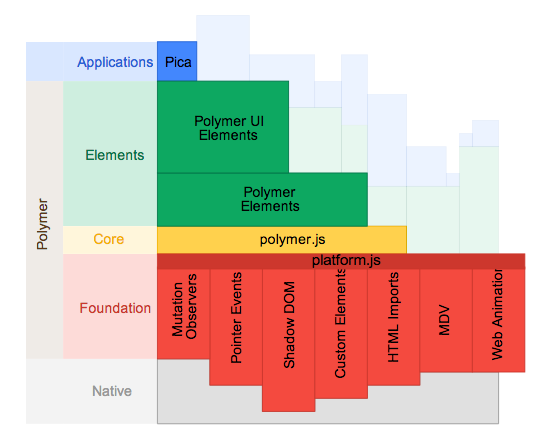
\includegraphics[width=\textwidth]{polymer_1}
\caption{Polymer Architecture}
\end {figure}
 

Web components standards provide the needed primitives to build new components. It is possible to build custom elements using these primitives, but it can be a lot of work.

The Polymer library provides a declarative syntax that makes it simpler to define custom elements. And it adds features like templating, two-way data binding and property observation to help developers build powerful, reusable elements with less code.

Custom elements. If users don’t want to write their own elements, there are a number of elements built with Polymer that it is possible to drop straight into existing pages. These elements depend on the Polymer library, but they can be used without using Polymer directly too.\cite{tch_polymer1}

Polymer is one of the first implementations of a user interface library built upon the Web Components standard.  Web Components are not fully supported by browsers, but they provide a polyfill library, webcomponents.js, that provides enough functionality to support Web Components and Polymer.

Web Components standard is the result of the evolution of user interface libraries over the past decade, finally reaching the goal of separating HTML, CSS and JavaScript and running HTML through W3C validators. For example, looking at a .css file, it is possbile to easily determine which selectors are actually used in HTML and especially programmatically used in JavaScript.  Similarly, JavaScript code is easy to organize so that code could be reused efficiently on multiple pages.\cite{tch_polymer2}

